\documentclass[11pt]{article}
\usepackage{fontspec}
\setmainfont{Arial}
\setsansfont{Arial}
\setmonofont{DejaVu Sans Mono}[Scale=MatchLowercase]
\usepackage[margin=1in]{geometry}
\usepackage{amsmath,amssymb}
\usepackage{graphicx}
\usepackage{booktabs}
\usepackage{array}
\usepackage{multirow}
\usepackage{siunitx}
\usepackage{caption}
\usepackage{subcaption}
\usepackage{placeins}
\usepackage{tikz}
\usetikzlibrary{arrows.meta,positioning,calc,fit,decorations.pathreplacing}
\usepackage[numbers,round]{natbib}
\usepackage[svgnames]{xcolor}
\usepackage{authblk}
\usepackage{microtype}
\usepackage{xurl}
\usepackage[hidelinks]{hyperref}

\captionsetup{font=small,labelfont=bf}
\setlength{\parskip}{0.3em plus 0.1em minus 0.05em}
\setlength{\parindent}{0pt}
\setlength{\emergencystretch}{1em}
\setlength{\textfloatsep}{10pt plus 3pt minus 3pt}
\setlength{\floatsep}{9pt plus 2pt minus 2pt}
\setlength{\intextsep}{9pt plus 2pt minus 2pt}
\renewcommand{\topfraction}{0.9}
\renewcommand{\bottomfraction}{0.85}
\renewcommand{\textfraction}{0.08}
\renewcommand{\floatpagefraction}{0.72}
\setcounter{topnumber}{3}
\setcounter{bottomnumber}{2}
\setcounter{totalnumber}{4}
\makeatletter
\setlength{\@fptop}{0pt}
\setlength{\@fpsep}{10pt plus 2pt}
\setlength{\@fpbot}{0pt plus 1fil}
\makeatother
\raggedbottom

\newcommand{\panfig}[1]{\resizebox{\textwidth}{!}{\input{#1}}}
\newcommand{\panhalffig}[1]{\resizebox{0.98\linewidth}{!}{\input{#1}}}

\graphicspath{{journal-figures/}{standalone-assets/}{tikz/}{./}}
\newcommand{\figpanel}[2]{Figure~\hyperref[#1]{\ref*{#1}#2}}
\newcommand{\InventoryFiles}{1587}
\newcommand{\LatentFiles}{1585}
\newcommand{\UniqueScores}{1236}
\newcommand{\NativeFiles}{910}
\newcommand{\NonNativeFiles}{675}
\newcommand{\ValidNativeFiles}{855}
\newcommand{\GuardedNativeFiles}{55}
\newcommand{\NullEligible}{60}
\newcommand{\NullCoherence}{59}
\newcommand{\NullJoint}{57}
\newcommand{\MaxExactDelta}{0.066412}

\hypersetup{pdftitle={Reference-anchored diagnostics of single-cell geometry and native allocation coherence},pdfauthor={Zeyu Fu}}
\title{Reference-anchored diagnostics of single-cell geometry and native allocation coherence}
\author[1]{Zeyu Fu*}
\affil[1]{\hspace{0.2em}State Key Laboratory of Trauma and Chemical Poisoning, Institute of Combined Injury,
Chongqing Engineering Research Center for Nanomedicine, College of Preventive Medicine,
Army Medical University, Chongqing, China\\\texttt{fuzeyu09@gmail.com}}
\date{}
\begin{document}
\maketitle

\begin{abstract}
Geometric preservation scores are often interpreted as evidence that a single-cell representation retains biological structure. We audited this interpretation using synthetic interventions, 24 stored representations, seven tissue sections and one blood sample. With a connected reference, reachability reduced to the fraction of candidate pairs in the same component; the identity held in all 322 applicable batteries. Global comparators responded to graded separation at smaller displacements than reachability. Most of the edge-survival increase with neighborhood size accompanied a rising permutation expectation, and candidate-specific correction changed representation orderings in 11 of 15 object--reference comparisons. On the tissue sections, corrected edge survival favored some embeddings, while separation showed no consistent ordering. Correlations with cortical-layer purity were descriptive and lacked independent donor replication. Native allocation coherence exceeded raw mixture and random smooth baselines, but matching mixture sharpness reduced its median advantage to 0.029 and favored the mixture in all three lung objects. These results support conditional measurement: geometric scores require their own chance expectations, established comparators and allocation baselines with matched sharpness. They do not establish biological preservation or universal method superiority.
\end{abstract}

\section{Introduction}

Low-dimensional representations are routinely used to summarize single-cell expression data, compare cell populations, and display gradual changes between transcriptional states~\cite{luecken2019practices,becht2019umap}. Their apparent simplicity creates a demanding measurement problem. A visually continuous path, a compact labelled group, and a probability vector that changes smoothly between neighbouring cells describe different properties. Each can be useful, yet none alone identifies the biological process that produced the observations. Evaluation therefore needs to specify both the object being measured and the relationship against which preservation is assessed. This study examines how that specification changes the interpretation of geometric scores through controlled coordinate interventions and remeasurement of fixed computational objects.

Neighbourhood preservation has a well-developed methodological basis. Trustworthiness and continuity assess intrusions and omissions in local neighbourhood rankings~\cite{venna2006local,venna2010retrieval}. Co-ranking summaries express related relationships across neighbourhood scales~\cite{lee2009quality}. Local linear embedding and Laplacian eigenmaps construct neighbourhood geometries of a different kind~\cite{roweis2000lle,belkin2003laplacian}, and t-distributed stochastic neighbour embedding (t-SNE) or uniform manifold approximation and projection (UMAP) coordinates are common visualization candidates rather than declared references~\cite{vandermaaten2008tsne,becht2019umap}. These approaches make locality explicit, which is valuable when nearby observations should remain nearby after projection. However, a question about the fate of a reference-connected pair is distinct from a question about the rank of an immediate neighbour. A small number of changed edges can separate large graph components while affecting relatively few local comparisons. The magnitude of that response is an empirical property of the graph and intervention, rather than a universal defect of a metric family.

Other evaluation traditions address complementary structures. Geodesic approaches use graph paths to represent relationships beyond immediate neighbours~\cite{tenenbaum2000global}, while inter-cluster reliability diagnostics examine changes in cluster organization~\cite{jeon2022steadiness}. In single-cell integration, evaluation also includes preservation of supplied biological annotations and trajectory-related ordering~\cite{luecken2022benchmarking}. Trajectory benchmarks distinguish topology, ordering and feature recovery as separate targets~\cite{saelens2019comparison}. Those annotations add information unavailable to a purely coordinate-based diagnostic. They also change the estimand: connectedness within a labelled group need not measure connectedness between groups, and agreement with an inferred ordering need not establish a biological lineage. A comparison is interpretable only when the graph construction, annotation inputs, and implementation identity are reported together with the score.

Tears and false neighbourhoods are the two elementary types of geometrical mapping distortion~\cite{lespinats2011checkviz}, and calibration by controlled damage offers a direct way to investigate how a score responds to each. Starting from the same reference, one can separate two arms, compress a branching coordinate, add noise, or break row correspondence while preserving the candidate marginal distribution. The intended intervention must nevertheless be isolated from incidental changes. If a damaged candidate removes the noise present in its comparator, an apparently favourable local response can combine denoising with structural damage. Likewise, a named software API and a locally implemented surrogate can behave differently even when both are described informally as trajectory conservation. Matched starting coordinates and direct upstream execution are therefore essential parts of a measurement experiment.

Probability-valued representations introduce an additional object-identity requirement. A native allocation vector assigns mass across defined coordinates of a model; an arbitrary continuous embedding does not become such an allocation merely because softmax makes its rows sum to one. For native allocations, Jensen--Shannon divergence~\cite{lin1991divergence} provides a bounded comparison between probability vectors. A smoothness ratio can compare divergence on reference edges with divergence among all cells, but its denominator determines the meaning and reproducibility of the result. Sampling positional pairs can introduce dependence on row order. Nearly uniform or constant allocations can also make a favourable ratio uninformative about useful between-cell variation.

{\looseness=1 Reference-anchored allocation geometry, abbreviated RAAG, addresses these questions with separately reported diagnostics. Reachability measures whether reference-connected pairs remain connected. Edge survival measures the hop distance between reference neighbours, and separation survival asks whether distant reference pairs remain separated relative to a candidate threshold. Allocation coherence compares local and overall probability variation only when native allocation semantics and operational dispersion checks are satisfied. Keeping these quantities separate makes their different failure responses visible. Their common reference is a declared coordinate representation. In the stored single-cell objects that representation is expression-derived; in the spatial case it is the tissue position of each spot. Neither choice asserts that the reference graph is biological ground truth or that every reference feature should be preserved.\par}

We evaluate this measurement design in two complementary settings. A small branching fixture supplies exact coordinate interventions, common initial noise, and explicit branch and pseudotime annotations for official metric calls. A fixed collection of saved representations supplies heterogeneous real-data computational objects whose identities, duplicate aliases, and allocation semantics can be traced. We then extend the analysis using a fixed subset to vary graph neighbourhood size, retained reference dimension, and the fraction of corrupted cell correspondences. These choices probe sensitivity within the observed inputs; they do not create new patients or independent biological experiments. All intervention levels and object-selection rules were fixed before these sensitivity scores were computed.

The study asks what evidence is needed before a geometric measurement can support a stated interpretation. We find that three ingredients are indispensable: the candidate-specific chance expectation of each score, a panel of established comparators evaluated under the same interventions, and a baseline that matches the smoothness or sharpness of the object being scored. With them, several conclusions that the raw scores suggest are reversed. Reachability becomes a check on the candidate graph's connectivity rather than a reference-anchored measure, edge survival's sensitivity to neighbourhood size shrinks to its corrected part, and comparisons between embeddings change once each is scored against its own null.

\section{Materials and Methods}

\subsection{Measurement workflow and analysis objects}

The coordinate input is a finite matrix $Z\in\mathbb R^{n\times q}$ paired row-for-row with a reference $X\in\mathbb R^{n\times d}$. The allocation pathway additionally requires model-declared probabilities $P\in\Delta^{K-1}$ for each cell; numeric normalization alone cannot supply that interpretation. Graph scores, allocation eligibility, dispersion and null comparisons remain separate outputs. No combined biological-success score is constructed. Preprocessing and the chosen reference define the question being asked, as they do elsewhere in single-cell analysis~\cite{luecken2019practices}. We call the implementation that produced the stored results the archived scorer; later sections compare it with an exact, identity-explicit reimplementation.

\subsection{Reference-anchored geometry}

Let $X=(x_i)_{i=1}^n$ be the reference and $Z=(z_i)_{i=1}^n$ the candidate, with the same cell identity in each row. On each space we construct the undirected union of a Euclidean $k$-nearest-neighbour graph, using $k=15$. Let $h_X(i,j)$ and $h_Z(i,j)$ denote unweighted shortest-path distances, with infinity for disconnected pairs. Let $\mathcal P_X=\{(i,j):i<j,\ h_X(i,j)<\infty\}$ and let $E_X$ be the undirected reference edges. Reachability and edge survival are
\begin{align}
 R(X,Z)&=\frac{1}{|\mathcal P_X|}\sum_{(i,j)\in\mathcal P_X}\mathbf 1[h_Z(i,j)<\infty],\label{eq:reachability}\\
 E(X,Z)&=\frac{1}{|E_X|}\sum_{(i,j)\in E_X}\frac{1}{h_Z(i,j)},\qquad 1/\infty=0.
\end{align}
The first counts connected pairs; the second measures local adjacency distortion. A small number of severed junction edges can disconnect many pairs. Conversely, a connected but randomly reordered candidate can have $R=1$, so $R$ alone is not a quality score. Neighbours use Euclidean distance and the union rather than intersection of directed neighbour lists, with $k'=\min(k,n-1)$ for a positive integer $k$ (the archived constructor additionally raises $k<1$ to one). Graph edges carry unit weight. Each unordered pair or edge enters its denominator once; the score formulas exclude self-pairs. The archived neighbour constructor drops the first returned rank, assuming it is the query itself. Exact duplicates can violate this assumption; the tie stress test below therefore delimits this implementation. Nonfinite inputs and reference populations with fewer than ten connected pairs are rejected instead of receiving a favourable score. The identity-explicit reimplementation described below reports no graph score when all rows of the reference or of the candidate are identical; the archived scorer still constructs a union nearest-neighbour graph on such input and can emit self-loops.

For separation survival, the reference far set $F_X$ contains the finite reference pairs whose hop distance is at least the 90th percentile $q_{0.9}$ of the finite values of $h_X$ (interpolated linearly at rank $1+0.9(N-1)$ among the $N$ sorted finite values); separation is withheld when $F_X$ has fewer than ten pairs. Let $m_Z$ be the median of the finite values of $h_Z$, the mean of the two central values when their number is even. We define
\begin{equation}
 S(X,Z)=\frac{1}{|F_X|}\sum_{(i,j)\in F_X}\mathbf 1[h_Z(i,j)\geq m_Z].
\end{equation}
Disconnected candidate pairs count as separated; the union graph of two or more rows always contains an edge, so the candidate always has a finite hop. This convention is complementary to reachability, but the candidate-dependent threshold also limits interpretation: $S$ is not an absolute distance-preservation measure. Graph construction, tied distances, $k$, and the chosen reference can change the answer. The baseline setting is $k=15$ with a 50-component reference. The additional sensitivity experiment varies $k$ and the retained reference dimension explicitly, over a finite grid described below.

\subsection{Chance expectations and tie-aware separation}

Uniformly permuting candidate rows while fixing the reference maps each distinct reference pair to a uniformly selected candidate pair. If the candidate graph is invariant to row relabelling, the exact expectations are
\begin{equation}
 E_0^{\rm exact}=\frac{1}{\binom n2}\sum_{i<j}\frac{1}{h_Z(i,j)},\qquad
 S_0^{\rm exact}=\frac{1}{\binom n2}\sum_{i<j}\mathbf 1[h_Z(i,j)\geq m_Z].
\end{equation}
Disconnected distances retain the conventions above. The scale and diversity chance-correction analyses use the means of 50 row-permutation draws, $E_0^{\rm MC}$ and $S_0^{\rm MC}$; the graded calibration and representation refits use the exact expectations. With the corresponding null denoted $E_0,S_0$, the corrected scores are
\begin{equation}
 E^*=\frac{E-E_0}{1-E_0},\qquad S^*=\frac{S-S_0}{1-S_0}.\label{eq:corrected}
\end{equation}
Correction is undefined when its null is one; such cases are not replaced by zero. In the 216 scale batteries, the largest Monte Carlo--exact discrepancies were 0.0014 for $E_0$ and 0.0054 for $S_0$. Candidate cutoff ties were absent in those arrays and in the regenerated diversity candidates. This check does not resolve ties in lattice-like tissue references under the archived neighbour constructor.

Integer-hop ties also affect the candidate-median threshold. The complementary far-versus-edge AUROC compares every reference far pair $f\in F_X$ with every reference edge $e\in E_X$:
\begin{equation}
 A_{FE}=\frac{1}{|F_X||E_X|}\sum_{f\in F_X}\sum_{e\in E_X}
 \left\{\mathbf 1[h_Z(f)>h_Z(e)]+\tfrac12\mathbf 1[h_Z(f)=h_Z(e)]\right\}.
\end{equation}
Infinite distances receive the highest tied rank, including half credit when both are infinite. The permutation expectation is 0.5. This is tie-aware rather than tie-free, and it does not by itself penalize all forms of fragmentation.

\subsection{Component partitions and global comparators}

When the reference is connected and the candidate component sizes are $n_c$, reachability reduces to a candidate-only statistic. Pair precision supplies the reverse conditional comparison:
\begin{equation}
 R=\frac{\sum_c\binom{n_c}{2}}{\binom n2},\qquad
 P_{\rm pair}=\frac{|\mathcal P_X\cap\mathcal P_Z|}{|\mathcal P_Z|}.\label{eq:component-pairs}
\end{equation}
The identity for $R$ is conditional on a connected reference; the precision is undefined if the candidate has no connected distinct pairs. On a connected reference $\mathcal P_X$ contains every distinct pair, so $P_{\rm pair}=1$ whenever it is defined; over-merging is therefore visible in $P_{\rm pair}$ and in the component ARI only against a fragmented reference. For the component contingency table $m_{uv}$, let $a_u=\sum_vm_{uv}$, $b_v=\sum_um_{uv}$, $M=\binom n2$, $A=\sum_u\binom{a_u}{2}$ and $B=\sum_v\binom{b_v}{2}$. The component adjusted Rand index~\cite{hubert1985comparing} is
\begin{equation}
 \operatorname{ARI}=\frac{\sum_{u,v}\binom{m_{uv}}{2}-AB/M}{(A+B)/2-AB/M}.
\end{equation}
The implementation assigns one to identical trivial partitions for which the denominator vanishes. These comparisons distinguish over-merging from preserved reference-pair recall.

Global comparators include Spearman correlation of all distinct-pair Euclidean distances, using average ranks for ties, and co-ranking summaries~\cite{lee2009quality}: the global quality $Q_{\rm global}$ and the log-weighted area under the rescaled co-ranking curve (AUC-RNX). For the ordered-pair co-ranking counts $q_{uv}$, where $u,v$ are reference and candidate neighbour ranks excluding self, define, for $1\leq K\leq n-2$,
\begin{equation}
 Q_{NX}(K)=\frac{1}{nK}\sum_{u=1}^K\sum_{v=1}^Kq_{uv},\qquad
 R_{NX}(K)=\frac{(n-1)Q_{NX}(K)-K}{n-1-K}.
\end{equation}
Let $K_{\max}$ be the smallest $K$ attaining the maximum of $Q_{NX}(K)-K/(n-1)$ on this grid, and $\mathcal K_>=\{K:K>K_{\max}\}$. The displayed implementation uses
\begin{equation}
 Q_{\rm global}=\frac{1}{|\mathcal K_>|}\sum_{K\in\mathcal K_>}Q_{NX}(K),\qquad
 \operatorname{AUC}_{RNX}=\frac{\sum_{K=1}^{n-2}R_{NX}(K)/K}{\sum_{K=1}^{n-2}1/K}.
\end{equation}
If $\mathcal K_>$ is empty, $Q_{\rm global}$ is the last available $Q_{NX}$. AUC-RNX is log-weighted, not an unweighted area. The comparator panel also retains trustworthiness, the local continuity meta-criterion (LCMC)~\cite{chen2009local}, and the zadu implementations~\cite{jeon2023zadu} of steadiness and cohesiveness~\cite{jeon2022steadiness}; the latter are randomized inter-cluster reliability diagnostics rather than RAAG graph scores.

\subsection{Graded calibration and paired responses}

The graded calibration uses the stored branching generator with candidate jitter drawn independently of the reference, alongside a cycle, a three-arm branch and three disjoint clusters. Separation amplitudes are zero, twelve logarithmically spaced values from 0.002 to 0.5, 2.5 and 9; centroid-merging fractions are 0, 0.5, 0.8, 0.9, 0.95, 0.97, 0.99 and 1. Each topology crosses $k\in\{5,15,30\}$, populations of approximately 450 and 2,000 rows, and 20 seeds. The original coupled-jitter branch is retained as a construction check. Within each seed $b$, the same jitter is retained across amplitudes $a$, so the mean paired response and its normalized display are
\begin{equation}
 \Delta_{b,s}(a)=s_b(a)-s_b(0),\qquad
 \bar\Delta_s(a)=\frac{1}{20}\sum_b\Delta_{b,s}(a),\qquad
 r_s(a)=\frac{\bar\Delta_s(a)}{\bar\Delta_s(9)}.
\end{equation}
Normalization is withheld for a zero full response. Ribbons show one seed standard deviation of $\Delta_{b,s}(a)$ divided by $|\bar\Delta_s(9)|$; full-response bars show one seed standard deviation without normalization. The descriptive response threshold is the first tested positive amplitude with the full-response sign and $|\bar\Delta_s(a)|>3\max\{\operatorname{SD}_b\Delta_{b,s}(a),10^{-12}\}$, also requiring a change greater than $10^{-9}$. It is a discrete repeatability rule, not a significance test or estimate of biological detection power. The marked neighbour radius is the saved median reference $k$th-neighbour distance.

\subsection{Exact coherence and applicability}

Allocation coherence requires a native allocation matrix $P$ with rows $p_i\in\Delta^{K-1}$ representing probabilities over the model's allocation coordinates. The Jensen--Shannon divergence~\cite{lin1991divergence} is computed in natural-log units after the implementation's fixed $10^{-12}$ clipping and row renormalization. Define
\begin{align}
 D_E &= |E_X|^{-1}\sum_{(i,j)\in E_X}\operatorname{JSD}(p_i,p_j),\\
 D_{\rm all} &= {\binom n2}^{-1}\sum_{i<j}\operatorname{JSD}(p_i,p_j),\\
 C_{\rm raw} &= \left[1-D_E/D_{\rm all}\right]_0^1.
\end{align}
For two allocation rows, with $m=(p+q)/2$,
\begin{equation}
 \operatorname{JSD}(p,q)=\frac12\sum_jp_j\log\frac{p_j}{m_j}
                         +\frac12\sum_jq_j\log\frac{q_j}{m_j}.
\end{equation}
The coherence denominator uses every unordered distinct pair in $D_{\rm all}$. The historical implementation sampled positional pairs using a fixed seed. Jointly reordering reference and allocation rows therefore changed the sampled denominator even though the scientific object was unchanged. Exact summation removes this sampling dependence, up to floating-point accumulation, at $O(n^2K)$ arithmetic cost. The implementation uses bounded row-block memory for the denominator; all-pairs graph distances still require quadratic storage. Unit tests compare the denominator with independently enumerated SciPy Jensen--Shannon distances and test joint row reordering.

On the clipped and renormalized rows, the normalized mean row perplexity is
\begin{equation}
 \Pi(P)=\frac{1}{nK}\sum_i\exp\!\left[-\sum_jp_{ij}\log p_{ij}\right].
\end{equation}
A denominator at or below $10^{-12}$ marks the allocation degenerate, and $\Pi(P)>0.95$ marks it near-uniform. Neither yields a quotable coherence value; the degenerate raw diagnostic is set to zero by convention. A constant uniform matrix satisfies both conditions and is classed as degenerate. The thresholds are declared operational guards, not estimated biological decision boundaries. Raw diagnostics remain available for auditing.

Continuous Gaussian coordinates are classed as non-native. A softmax of these coordinates is tabulated separately from native coherence; its dimension is the number of latent coordinates, which is 10 for the stored mixture-regularized representations, not their mixture truncation of 50. That transformation is not a posterior responsibility matrix and cannot support allocation claims. The inventory and all reported re-scores declare allocation semantics explicitly instead of inferring them from the numerical values.

\subsection{Reference-aware allocation baselines and conditional uncertainty}

This analysis preserves negative coherence rather than clipping it. For an eligible nonconstant allocation, it reports
\begin{equation}
 C_{\rm unc}=1-D_E/D_{\rm all},\qquad
 z_C=\frac{C_{\rm unc}-\bar C_{\pi}}{\operatorname{SD}(C_{\pi})}.
\end{equation}
Here $\bar C_{\pi}$ and its sample standard deviation use 200 row permutations per native object. This descriptive standardized distance is not a Gaussian-test statistic. These draws are separate from the 999-draw fixed-object analysis defined below.

Reference-aware baselines fit ten-component Gaussian mixtures directly to $X$, with diagonal covariance on all 50 reference principal components (PCs) or full covariance on the first ten. The fits use three initializations, seed 0 and covariance regularization $10^{-6}$. Their responsibilities are
\begin{equation}
 r_{ij}=\frac{\omega_j\,\varphi(x_i;\mu_j,\Sigma_j)}{\sum_\ell\omega_\ell\,\varphi(x_i;\mu_\ell,\Sigma_\ell)},\qquad
 r_{ij}^{(T)}=\frac{\exp(\log r_{ij}/T)}{\sum_\ell\exp(\log r_{i\ell}/T)}.
\end{equation}
The second expression is followed by the fixed simplex clipping and renormalization. Bisection selects $T$ so that $\Pi(r^{(T)})=\Pi(P)$, matching mean row perplexity rather than biological semantics. The full-covariance ten-PC mixture is the displayed sharpness-matched baseline; diagonal ten- and twenty-component variants remain in the saved sensitivity record.

Twenty random smooth baselines use a single global reference scale $\sigma_X=\operatorname{SD}(\{x_{i\ell}\}_{i,\ell})$, not feature-wise standardization:
\begin{equation}
 p^{\rm rand}_{ij}=\operatorname{softmax}_j\!\left(\beta\,(X/\sigma_X)W\right)_i,\qquad
 W_{\ell j}\sim\mathcal N(0,1/d),\quad j=1,\ldots,10.
\end{equation}
Each matrix uses an independent saved random draw; $\beta$ is either one or is selected to match native mean perplexity. Gaussian-mixture and random responsibilities are positive numerical baselines, not declarations that they share the native model's allocation meaning.

For comparison with graph smoothness, the global squared-Euclidean multivariate Geary ratio~\cite{geary1954contiguity}, the global counterpart of the local multivariate form~\cite{anselin2019local}, uses the same undirected reference edges:
\begin{equation}
 c(P)=\frac{(n-1)\sum_{(i,j)\in E_X}\lVert p_i-p_j\rVert_2^2}
 {2|E_X|\sum_i\lVert p_i-\bar p\rVert_2^2}.
\end{equation}
Replacing Jensen--Shannon divergence by squared Euclidean distance in $C_{\rm unc}$ gives $1-c$ exactly. Their empirical association does not make the two divergences identical.

The saved paired bootstrap holds the graph and all fitted allocations fixed. For each of 1,000 draws, cell multiplicities $w\sim\operatorname{Multinomial}(n;1/n,\ldots,1/n)$ give
\begin{align}
 D_E(w)&=\frac{\sum_{(i,j)\in E_X}w_iw_j\operatorname{JSD}(p_i,p_j)}{\sum_{(i,j)\in E_X}w_iw_j},\\
 D_{\rm all}(w)&=\frac{\sum_{i\ne j}w_iw_j\operatorname{JSD}(p_i,p_j)}{(\sum_iw_i)^2-\sum_iw_i^2}.
\end{align}
Thus repeated copies of the same original cell are excluded from the all-pair denominator. The same weights are used for native and raw-baseline coherence, and their difference uses the 2.5th and 97.5th percentiles. Random-baseline coherence is first averaged over its twenty maps. These are graph-conditional intervals, without refitting or donor resampling; no bootstrap interval was computed for the subsequently tempered mixtures.

\subsection{Independent absolute-variation stress fixture}

An independent numerical fixture tests whether relative coherence establishes substantial absolute allocation variation. It uses 32 cells with reference coordinate $x_i=i/31$, $i=0,\ldots,31$, and $k=5$. Nine-coordinate tail probabilities are $q_{ij}=((31-i)(j+1)+i(9-j))/(31\cdot45)$, $j=0,\ldots,8$, and ten-coordinate allocations are $p_i=(1-\epsilon,\epsilon q_i)$. The primary tail masses are $1,10^{-1},\ldots,10^{-14},0$; nine additional prespecified values bracket the clipping and ideal denominator boundaries. Five controls use smooth tails, tails reassigned by the bijection $(13i+7)\bmod32$, alternating vertices, constant tails, and uniform tails. One varying near-uniform control completes 126 recorded cases. Reassignment retains recipient identities and the probability-row multiset.

The identity-explicit numerical implementation is compared with an independent 80-digit decimal calculation on the same delivered, clipped and normalized probabilities. The saved full validation passes all 19 software tests and all fixture comparisons, with no skipped tests. These are separately checked numerical fixtures, not remeasurements of the historical inventory or the 444 stored-object batteries. For ideal unclipped inputs, all-pair Jensen--Shannon divergence scales as $D_{\rm all}(p)=\epsilon D_{\rm all}(q)$, while relative coherence is unchanged. Clipping can break that identity at small tail mass. Eligibility requires the implemented denominator and dispersion guards, but does not impose a biologically meaningful absolute-variation threshold. The complementary absolute diagnostic is mean pairwise total variation,
\begin{equation}
 \overline{\operatorname{TV}}(P)=\frac{1}{\binom n2}\sum_{i<j}\frac12\lVert p_i-p_j\rVert_1.
\end{equation}



\subsection{Matched-noise calibration and upstream identity}

The synthetic reference contains 450 points in two dimensions: a 150-point trunk and two 150-point arms. Reference coordinates include independent Gaussian noise with standard deviation 0.004. A faithful candidate adds noise with standard deviation 0.01 and is therefore not an isometric copy of the reference. Every damage intervention begins with that same faithful realization. We translate the two arms by opposing vertical shifts of 0.5, 2.5, or 9; retain 0.5 or 0 of the fork coordinate for collapse; add noise of standard deviation 0.06 or 0.18; or permute candidate rows. Identity and a rotation/uniform rescaling of faithful provide controls. Seeds 7, 17, and 42 each yield 12 candidates, including the historical unmatched shatter as a separately named diagnostic. Reference and faithful jitter generators share the fixture seed, so their initial draws are coupled; the three seeds are paired fixture realizations, not independent biological samples. The sweep is exploratory, not a confirmatory test.

We run canonical local-rank and graph metrics, the zadu implementations including steadiness and cohesiveness, and RAAG. The official single-cell integration benchmarking package (scIB) version 1.1.7 is called directly through both public APIs~\cite{scib2025software}. Scanpy~\cite{wolf2018scanpy} constructs the candidate neighbour graph from the candidate embedding with 15 neighbours. Synthetic branch labels and known pseudotime are supplied as cell annotations; the trajectory API computes diffusion pseudotime internally~\cite{haghverdi2016diffusion}. There is no batch covariate. This is an explicit synthetic stress test of those API inputs, not a complete integration benchmark.

The three-coordinate allocation controls use the same branching reference. Before clipping, trunk cells have $q_i=e_0$ and arm-$b$ cells have $q_i=(1-a_i)e_0+a_ie_b$, with $a_i=\max\{0,\min(1,2t_i-1)\}$ and known pseudotime $t_i$. Clipping below at $10^{-6}$ and renormalizing gives the smooth rows $\widetilde q_i$. Sharp, diffuse and near-uniform rows are obtained from these smooth rows by powers $\gamma=4$, $0.15$ and $0.02$, respectively:
\begin{equation}
 p_{ij}^{(\gamma)}=\frac{\widetilde q_{ij}^{\gamma}}{\sum_\ell\widetilde q_{i\ell}^{\gamma}}.
\end{equation}
The implementation applies the fixed $10^{-12}$ clipping and renormalization to each powered row. Shuffled controls reassign the smooth rows using the fixture seed; constant controls repeat their mean row. All six controls are declared native probabilities, allowing raw coherence, perplexity and all-pair divergence to be compared without assigning allocation meaning to continuous coordinates.

\subsection{Local rank scores and annotation-dependent comparators}

Let $N_X^k(i)$ and $N_Z^k(i)$ be directed Euclidean neighbour lists, excluding the query, and let $r_X(i,j)$ be the one-based reference rank. Trustworthiness penalizes candidate neighbours outside the reference neighbourhood~\cite{venna2006local,venna2010retrieval}:
\begin{equation}
 T_k=1-\frac{2}{nk(2n-3k-1)}\sum_i\sum_{j\in N_Z^k(i)\setminus N_X^k(i)}(r_X(i,j)-k).
\end{equation}
The calibration uses the scikit-learn implementation~\cite{pedregosa2011scikit} with $k=15<n/2$. The local continuity meta-criterion subtracts the expected random overlap from the neighbourhood overlap~\cite{chen2009local,lee2009quality}:
\begin{equation}
 \operatorname{LCMC}_k=\frac{1}{nk}\sum_i|N_X^k(i)\cap N_Z^k(i)|-\frac{k}{n-1}.
\end{equation}
Its identity value is $1-k/(n-1)$, not one. The stored calibration record holds the zadu implementation of this quantity; the graded calibration evaluates it from the co-ranking matrix. The response plots report $100(s_{\rm damaged}-s_{\rm faithful})$ in percentage points for each paired fixture seed; these are score differences, not inferred detection probabilities. Other historical and upstream stack outputs remain identified in the complete calibration record and are not interchangeable with these two displayed quantities.

For the local root-geodesic surrogate, let $g_X$ and $g_Z$ denote shortest paths on the distance-weighted union neighbour graphs, $r=\arg\min_i t_i$, and $\Omega=\{i:g_X(r,i),g_Z(r,i)<\infty\}$. Its reported value is
\begin{equation}
 C_{\rm root}=\frac{1+\rho_{\rm S}((g_X(r,i))_{i\in\Omega},(g_Z(r,i))_{i\in\Omega})}{2},
\end{equation}
where $\rho_{\rm S}$ is Spearman correlation with average ranks for ties. At least three reachable rows are required. This conditional, unpenalized score uses Euclidean edge lengths, unlike RAAG's unweighted hop distances; the separately saved component-penalized variant is not the displayed surrogate. The graph is built by the archived neighbour constructor with $k\geq2$.

Official scIB graph connectivity averages the largest within-label component fractions~\cite{scib2025software,luecken2022benchmarking}. With supplied label classes $\mathcal L$ and the Scanpy candidate connectivity graph $G_Z$, it is
\begin{equation}
 \operatorname{GC}=\frac{1}{|\mathcal L|}\sum_{\ell\in\mathcal L}
  \frac{|\operatorname{LCC}(G_Z[\ell])|}{|\ell|}.
\end{equation}
The official trajectory score instead compares known reference pseudotime $t$ with the API-produced diffusion pseudotime $\widehat t$~\cite{scib2025software,haghverdi2016diffusion}:
\begin{equation}
 C_{\rm scIB}=\frac{1+\rho_{\rm S}(t,\widehat t)}{2}.
\end{equation}
The API keeps cells with supplied pseudotime, takes the label with the lowest mean pseudotime over all those cells, selects a root among that label's cells inside the largest candidate component using three diffusion coordinates, and computes diffusion pseudotime in that component. Missing values outside it and diffusion values greater than one are set to zero before correlation; failure to find a root returns zero under the upstream convention. The calibration supplies no batch key. This graph, root rule and zero handling are not the local surrogate's reachable-row filtering. Every stack result retains warnings, exceptions or nonfinite status, and failed official calls are never replaced by a surrogate.

To locate the source of the low identity-control value, the official routine was rerun on the saved fixture arrays of all three seeds. For every candidate we recorded the root cell that the official heuristic selects. When the candidate graph had a single component we also recomputed diffusion pseudotime from the cell with the smallest known pseudotime, which at the default settings reproduces the official identity values to within 0.0005, and computed the Spearman correlation between known and recomputed diffusion pseudotime within each branch; disconnected candidates retain only the official score, the selected root and the component sizes. For the identity control we then varied one setting of this recomputation at a time: the number of diffusion components used by the pseudotime step (3, 4 or the default 10), the neighbour count of the Scanpy graph (15 or 30), and added Gaussian jitter with standard deviation 0.002, 0.006 or 0.01 (five draws per seed and level, with fixed random seeds).



\subsection{Historical inventory and permutation comparison}

The inventory includes every stored array file in a fixed collection of earlier computational outputs. It finds \InventoryFiles{} files, including \LatentFiles{} latent arrays with valid stored test indices and two non-latent containers. Computation identity includes the dataset, the stored test indices, the latent array and its semantic allocation type. This retains every file alias while reducing scoring to \UniqueScores{} distinct objects. Neither aliases nor repeated checkpoints are treated as independent observations. Aggregate results without a saved latent array in this collection are outside the re-score coverage.

Four stored expression caches are used only after they match their recorded input specifications; the reconstructed normalized matrix must also match its recorded specification. PCA with 50 components and seed 42 is fitted on the actual stored test indices, producing 14 dataset/index reference objects. This reproduces the historical, transductive expression-reference estimand; it does not turn the old preprocessing into training-only preprocessing. The stored backgrounds are hematopoiesis~\cite{setty2019palantir}, dentate gyrus~\cite{hochgerner2018conserved}, pancreatic endocrinogenesis~\cite{bastidas2019endocrinogenesis}, and adult lung tissue~\cite{vieirabraga2019lung}. The lung accession GSE130148 contains uninvolved parenchyma from tumour-resection material of four patients~\cite{lung_geo130148}; the historical cell-random splits are not patient holdouts. Organ annotations and inferred fate probabilities have different provenance from biological ground truth.

For the historical focused 144-run manifest we retain every run and ten row permutations per run, using seed 0. A permutation preserves the latent marginal distribution while destroying correspondence to reference rows. We report whether the observed score exceeds the maximum of those ten values. This is descriptive: the smallest Monte Carlo permutation $p$-value with the observed arrangement included is $1/11\approx0.091$~\cite{phipson2010permutation}. These comparisons do not establish 5\% significance, and native coherence uses only eligible native rows.

\subsection{Two references and five representations}

The extension asks the same geometry scores on two declared references. For tissue sections the reference is the stored two-dimensional position. For the same sections, and for one dissociated blood sample, a second reference is the 50-component expression PCA. Objects were fixed before scores were read: the St{\aa}hl olfactory-bulb section~\cite{stahl2016spatial}; dorsolateral prefrontal cortex (PFC) sections 151673 and 151507 from the Lieber Institute for Brain Development~\cite{maynard2021dlpfc}; breast-cancer liver-metastasis sample A\_0069226~\cite{chan2026bclm}; the 10x Genomics Visium demonstrations of human lymph node~\cite{tenxlymph}, breast cancer~\cite{tenxbreast}, and ovarian cancer~\cite{tenxovary}; and the 10x Genomics count matrix of 3,000 peripheral-blood mononuclear cells (PBMC)~\cite{tenxpbmc3k,zheng2017massively}. Spots outside tissue are excluded. Genes seen in fewer than three spots are removed, counts are library-size normalized and log-transformed, and the 2{,}000 most variable genes are kept.

The compared representations are that PCA (seed 42), a 10-dimensional scVI latent of the same counts~\cite{lopez2018scvi,gayoso2022scvitools}, a two-dimensional UMAP of the PCA neighbourhood graph~\cite{becht2019umap}, a 10-dimensional Gaussian random projection of the scaled genes (seed 0), and one permutation of the PCA rows (seed 0). scVI uses one hidden layer, a negative-binomial likelihood, and at most 200 epochs on one GPU. The neighbour count remains 15. Native coherence is not quoted. Repeating the tissue coordinates as a candidate scores 1 and is only a scorer check. When the reference is the PCA, the PCA candidate scores 1 by construction.

For clarity, the representative transformations are stated explicitly. After the gene-detection filter and removal of zero-library rows, counts $c_{ig}$ are transformed to $b_{ig}=\log(1+10^4c_{ig}/\sum_gc_{ig})$. The selected variable genes are standardized with Scanpy and clipped at its magnitude limit of 10, giving matrix $A$. If $A_c$ is its column-centered form and $V_d$ its first $d=\min(50,n-1,G-1)$ right singular vectors, the three linear candidates are
\begin{equation}
 Z_{\rm PCA}=A_cV_d,\qquad Z_{\rm RP}=AW,\qquad Z_{\rm perm}=\mathsf P_\pi Z_{\rm PCA},
\end{equation}
where $G$ is the retained gene count, $W_{g\ell}\sim\mathcal N(0,1)$ has ten columns, and $\mathsf P_\pi$ permutes rows without changing their values. The implemented random projection has no additional variance normalization. PCA and its expression reference use every retained component for scoring, not only the two displayed coordinates.

UMAP uses the Scanpy fuzzy neighbour graph of the PCA, with membership weights $w_{ij}$, rather than RAAG's binary union graph. Its representative layout objective is fuzzy cross-entropy~\cite{mcinnes2018umap}:
\begin{equation}
 \mathcal L_{\rm UMAP}=-\sum_{i<j}\left[w_{ij}\log v_{ij}+(1-w_{ij})\log(1-v_{ij})\right],
\end{equation}
with $v_{ij}=(1+a\lVert y_i-y_j\rVert^{2b})^{-1}$ for two-dimensional coordinates $y_i$. The library fits $a,b$ from its distance parameters and uses stochastic optimization with negative sampling, so this equation describes the layout target rather than a claim of exact all-pair optimization. The PCA neighbour graph and UMAP use seed 0.

For the configured scVI model, a standard-normal latent $u_i\in\mathbb R^{10}$ decodes retained raw counts through a negative-binomial observation model~\cite{lopez2018scvi,gayoso2022scvitools}:
\begin{align}
 u_i&\sim\mathcal N(0,I_{10}),\qquad c_{ig}\mid u_i,\ell_i\sim\operatorname{NB}(\ell_i f_{\theta,g}(u_i),\vartheta_g),\\
 \mathcal E_i&=\mathbb E_{q_\phi(u_i\mid c_i)}\!\left[\sum_g\log p_\theta(c_{ig}\mid u_i,\ell_i)\right]
 -\operatorname{KL}\!\left(q_\phi(u_i\mid c_i)\,\|\,\mathcal N(0,I_{10})\right).
\end{align}
Here $\ell_i$ is the observed library size over retained genes, $f_\theta$ has nonnegative gene frequencies summing to one, and $\vartheta_g$ is gene-specific inverse dispersion. Training optimizes the evidence lower bound using the library's KL warm-up and early stopping within the stated budget, with seed 0. Scored coordinates are posterior means, $z_i=\mathbb E_{q_\phi}[u_i]$, not decoder gene probabilities or native allocation vectors. The scVI scatter views retain its first two latent coordinates. Those views come from a separate refit with the same seed and budget; the heatmaps retain the original saved scores, and the displayed coordinates need not equal the scored arrays.


\subsection{Representation refits and candidate-neighbour layer purity}

The diversity arrays used for chance correction were regenerated under the archived preprocessing and training recipe. Of 75 raw geometry-score triples, 73 reproduced the archived triple exactly. Both exceptions involved UMAP on the same prefrontal section: tissue-reference edge survival and separation were 0.2116 and 0.8077 rather than 0.2076 and 0.7512, and expression-reference values were 0.2679 and 0.9848 rather than 0.2654 and 0.9953. Reachability was unchanged. Chance-correction analyses use the regenerated arrays, whereas the earlier raw-score tables and coordinate-summary heatmaps retain their archived records. The two records are not treated as interchangeable.

On the bulb and both prefrontal sections, scVI and UMAP were refitted with seeds 0--4 while the PCA and its neighbour graph remained fixed. The same retained rows, counts and budget were used, without donor splitting or a new training-budget comparison. For each prefrontal section, externally supplied cortical-layer annotations are matched to barcodes. Among the labelled rows $\mathcal L$, a new 15-neighbour graph is built separately in each candidate, excluding the query. Candidate-neighbour layer purity is
\begin{equation}
 U_{\rm layer}(Z)=\frac{1}{15|\mathcal L|}\sum_{i\in\mathcal L}
 \sum_{j\in N^{15}_{Z,\mathcal L}(i)}\mathbf 1[\ell_i=\ell_j].
\end{equation}
Unlabelled rows are removed before finding neighbours; tissue neighbours are not used in this purity. Thirteen arrays per section are displayed: five scVI, five UMAP, and one each of PCA, random projection and permuted PCA. Descriptive Spearman associations exclude permuted PCA and use twelve arrays. Refit seeds are algorithmic repeats, not independent methods, sections or donors. The labels are external to expression fitting, but are annotations of the same tissue object rather than independent biological validation.

\subsection{Scale and correspondence experiments}

Selection, settings, corruption seeds and output quantities were fixed before these sensitivity scores were computed. The selected representations use the same four backgrounds (labelled blood, dentate, pancreas and lung in the figures), stored seeds 0, 1, and 2, and ten coordinates. Each has 450 test rows, except pancreatic endocrinogenesis with 381. Within each background the reference and test rows are shared across the three stored seeds and both representation types. Native objects were trained under a symmetric concentration-one allocation prior; continuous objects used a mixture penalty of weight one with truncation 50. They are selected by these configuration names, without inspecting their scores. Their role here is to supply probability-valued and continuous computational objects, not to estimate a difference in model effectiveness. The stored inputs preserve the matched test indices and the full selected latent and reference arrays.

For graph sensitivity, each object is scored at all nine combinations of three neighbour counts and three retained reference ranks. For correspondence sensitivity, a seeded permutation chooses a nested subset of $\lfloor fn\rfloor$ cells at each fraction $f\in\{0,0.1,0.25,0.5,1\}$. Their allocation rows are reassigned in a single cycle. Fractions select nested sets, but their cycle assignments differ. Corruption seeds are 0, 17, and 42; the exact changed fractions are recorded. The allocation marginal distribution is unchanged, and the reference is fixed. Geometry and applicable exact coherence are recomputed after each intervention.

A subsequent, separately declared paired-grid audit subtracts the continuous-coordinate score from the native-allocation score for each background--seed pair at every one of the nine $k/d$ settings. We record strict sign reversals relative to $(k,d)=(15,50)$, exact ties, and within-pair difference ranges for reachability, edge survival, and separation. The twelve pairs are selected computational objects, not donors or a randomized comparison of methods; unlike the within-object scale analysis, their candidate representations also differ in model, training, and semantic type. These contrasts test whether a descriptive ordering is sensitive to the measurement setting, not which model is superior.

Separately from the historical 144-run comparison with ten permutations, a fixed-object analysis tests exactly twelve eligible native arrays at the baseline setting. For each, it holds the reference graph and allocation-row multiset fixed, generates 999 independent random row orders with a recorded PCG64 seed reset per object, and reassigns allocation rows before computing exact coherence. Precomputed pairwise Jensen--Shannon distances preserve the all-distinct-pair denominator. The unpermuted score is checked against the stored battery to $10^{-12}$. With null ties counted against the observed score, the one-sided Monte Carlo probability is
\begin{equation}
 p_{\rm MC}=\frac{1+\sum_{b=1}^{B}\mathbf 1[C_b\geq C_{\rm observed}]}{B+1},\qquad B=999.
\end{equation}
This tests row correspondence under that exchangeability null, not a population-level biological hypothesis; the across-object adjustment is the post hoc Holm correction described below.

The invariance controls use one fixed orthogonal transform followed by scaling by 2.5, and one fixed joint row permutation per object. Geometry uses the rotated continuous coordinates directly; allocation coherence is not interpreted for the rotated arrays. Joint row permutation retains the original semantic declaration. All 444 batteries run on CPU with at most two numerical threads and no optimizer updates. Complete rows, unavailable values and elapsed execution time are retained. Summaries are descriptive; neither the grid settings nor the corrupted copies are treated as independent experimental units.

\subsection{Independent recomputation and statistical scope}

A post hoc robustness audit recomputes the 216 graph-grid results without importing the archived scorer. It explicitly removes self-distances, sorts pair distances, forms union graphs and computes shortest paths in a separate SciPy implementation~\cite{virtanen2020scipy}. Exact ties at the neighbour cutoff are counted because they can make neighbour identity depend on tie handling. Native coherence is independently evaluated from a full Jensen--Shannon matrix; its constant distinct-pair denominator allows fast permutation of row indices. We reproduce the archived 999-draw stream and run a second stream with seed 104729, reinitialized separately for each of the twelve native objects. Each stream retains its own $(b+1)/(999+1)$ probability, with $b$ counting null scores greater than or equal to the observed score~\cite{phipson2010permutation}; streams are not retrospectively pooled.

The audit also reports a post hoc Holm correction for the twelve original fixed-object probabilities~\cite{holm1979sequential}. For sorted probabilities $p_{(i)}$, the adjusted value is
\begin{equation}
 p^{\rm Holm}_{(i)}=\min\!\left\{1,\max_{j\leq i}(12-j+1)p_{(j)}\right\}.
\end{equation}
This family is limited to the twelve baseline native-coherence tests, excluding other metrics and the separate historical 144-run inventory. Such correction addresses this declared multiplicity, not exchangeability of donors, selection of datasets or population generalization. The same saved cells, graph settings and algorithmic seeds cannot provide independent biological replication~\cite{zimmerman2021pseudoreplication}.

A final recomputation uses a second, identity-explicit implementation of the same scores. It requires ordered persistent cell identities, excludes each diagonal explicitly, completes every neighbour-cutoff tie group before an identity-based choice, and sums row totals with compensated arithmetic. Here the identities are the saved test indices within each dataset: computational identities, not recovered barcodes. It re-scores the 216 scale settings, the 180 correspondence perturbations, the 48 invariance controls and both 999-draw streams. Tolerances were fixed before execution: $10^{-12}$ for geometry scores, $10^{-10}$ for coherence, and exact equality for pair, edge and hop counts, eligibility flags and permutation tail counts. Recipient rows keep their identities when allocation rows are reassigned, whereas the joint reorder moves rows and identities together. Agreement of two implementations on these objects is a numerical check, not a biological validation.

An additional synthetic stress test deliberately violates the no-tie setting: twenty candidate rows have the same three-dimensional zero coordinate, paired with Gaussian reference rows generated with seed 91. At $k=5$ we count self-loops and jointly reorder both matrices with seeds 0, 17 and 42. This probes exact coordinate collapse; it is separate from the 24 stored objects and does not silently replace their stored scorer or results.

Tissue references have a different tie structure. Visium spot positions are integer pixel coordinates on a lattice, so the fifteenth and sixteenth nearest tissue neighbours are exactly equidistant for 2.6--41.4\% of the spots in six of the seven sections (none in the olfactory-bulb section). The tied group has two spots, except on the liver-metastasis section, where it reaches four, and the archived constructor then chooses among the tied spots by array position. Candidate graphs and expression references have no such ties. Every tissue-reference comparison was therefore rescored against 62 reference graphs per section: the archived constructor in the saved order; the archived constructor after each of 30 random reorderings of the reference rows, with the resulting edges mapped back to the original cell identities (candidate graphs stay in the saved order and have no cutoff ties); 30 random breaks of every cutoff tie group; and one tie-complete graph that keeps every strictly nearer neighbour and every neighbour at the cutoff distance, so a spot can have more than $k$ directed neighbours. Random draws used fixed seeds, and the saved-order scores reproduce the stored scores exactly.

\subsection{Figure summaries and display conventions}

For a declared group $\mathcal G$ of saved computations, mean scores and baseline changes are
\begin{equation}
 \bar s_{\mathcal G}(k,d)=\frac{1}{|\mathcal G|}\sum_{u\in\mathcal G}s_u(k,d),\qquad
 \Delta\bar s_{\mathcal G}(k,d)=\bar s_{\mathcal G}(k,d)-\bar s_{\mathcal G}(15,50).
\end{equation}
The scale heatmaps average three stored model seeds and show absolute reachability but changes for the other diagnostics. Correspondence curves first average three corruption seeds within a model seed; their thick curves then average the three model seeds within a background, while faint curves retain model-seed means. Historical permutation margins are $M_u=C_u-\max_{1\leq b\leq10}C_{u,b}$; ordering these margins changes their display position, not their value or denominator. Count bars distinguish file aliases, distinct objects and eligible focused runs.

Heatmap colours retain unrounded values; numeric annotations round to two decimals, with scale-setting changes of magnitude below 0.005 printed as zero. Separate signed colour limits are used for different diagnostics, while absolute scores use zero to one. Probability-variation panels use the stated square-root or logarithmic display axes without transforming the score definition. Coordinate plots retain equal aspect, all exported rows and data-derived limits; axes using thousands of tissue-coordinate units state the scaling. Colour denotes expression PC 1 with a separate range per specimen. No unavailable modality is imputed, continuous candidates do not enter native coherence, and schematic glyphs represent workflow components rather than measurements. Figures and tables are presented in Results; these conventions define how their saved measurements are displayed.



\subsection{Ethics and computational assistance}
This study reanalyzed synthetic fixtures and previously published public single-cell and spatial transcriptomics datasets. No new participants were recruited and no human or animal specimens were collected. Ethical oversight and consent for the original measurements are described by the source studies; no new institutional approval or exemption is claimed here.
AI-assisted tools supported manuscript editing and computational checks. The author is responsible for the scientific interpretation and final text.

\section{Results}

The measurement quantities operate on different input relationships, summarized in Table~\ref{tab:estimands}. Matched coordinate graphs supply three separate diagnostics (Supplementary Fig.~S1); native probabilities enter a distinct coherence pathway with eligibility guards (Supplementary Fig.~S1). Reference and correspondence probes retain fixed objects (Supplementary Fig.~S1), as do the null and invariance controls (Supplementary Fig.~S1). The comparison preserves the distinction between coordinate diagnostics, native probability allocations, and metrics that require supplied annotations. A root-geodesic surrogate and the official scIB trajectory metric are different computations and are reported separately.

\begin{table}[tbp]
\centering\small
\caption{Measurement objects and scope. No entry alone identifies biological lineage truth. The local surrogate and official scIB trajectory metric are distinct computations.}
\label{tab:estimands}
\begin{tabular}{>{\raggedright\arraybackslash}p{0.25\linewidth}>{\raggedright\arraybackslash}p{0.31\linewidth}>{\raggedright\arraybackslash}p{0.34\linewidth}}
\toprule
Quantity & Input relationship & Permitted interpretation\\
\midrule
RAAG $R,E,S$ & Matched candidate/reference rows & Coordinate graph preservation relative to that reference\\
Native coherence & Reference edges and native simplex probabilities & Allocation smoothness relative to nonlocal allocation variation\\
Local root surrogate & Reference and candidate root distances on reachable rows & Conditional rank agreement of graph distances\\
Official scIB connectivity & Candidate graph and supplied branch labels & Within-label connectedness\\
Official scIB trajectory & Known pseudotime, labels, candidate graph & Conservation of an annotation-derived ordering by diffusion pseudotime\\
\bottomrule
\end{tabular}
\end{table}





\subsection{Matched-noise calibration separates confounding from disconnection}

The faithful candidate retains its initial jitter (\figpanel{fig:interventions}{a}). Opposing arm translations separate the branches (\figpanel{fig:interventions}{b--c}), fork projection removes their vertical distinction (\figpanel{fig:interventions}{d}), additional noise disperses the coordinates (\figpanel{fig:interventions}{e}), and row permutation changes the coordinate-to-cell assignment (\figpanel{fig:interventions}{f}). Supplementary Table~S1 gives the seed-42 scores. Trustworthiness and LCMC retain small local responses, whereas reachability records loss of connected pairs and edge survival changes little. The complete calibration record includes all 36 candidates and all metric stacks. Differences across these seeds describe fixture repeatability, not biological replication or statistical power.

\begin{figure}[tbp]
\centering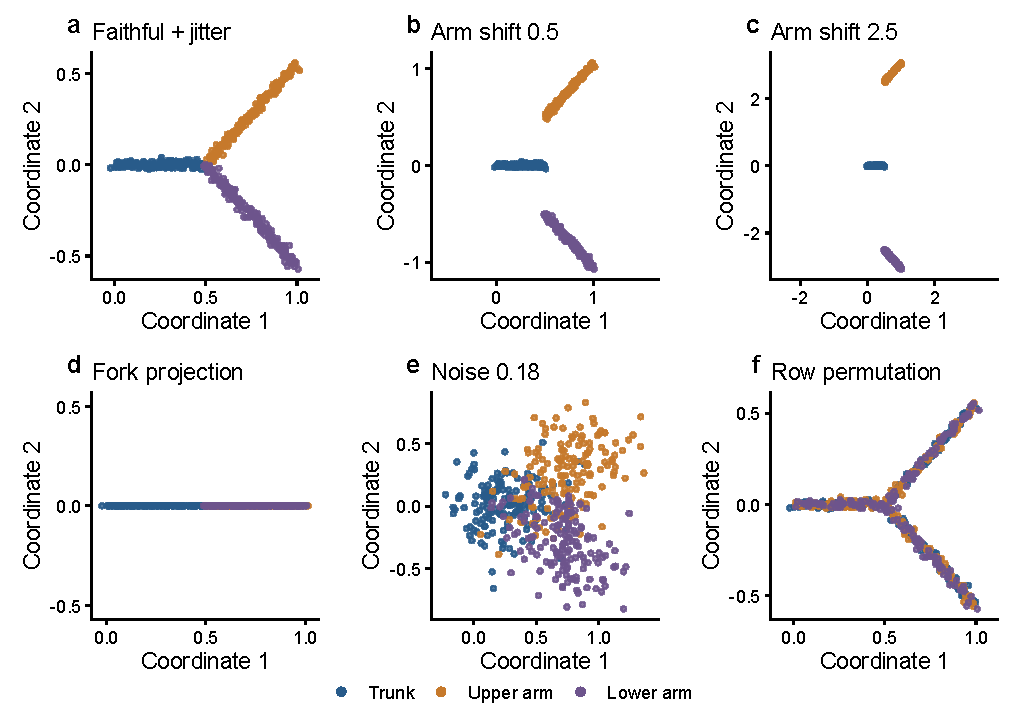
\includegraphics[width=\linewidth,height=0.64\textheight,keepaspectratio]{journal-figures/calibration_perturbations.pdf}
\caption{Matched-noise coordinate interventions for fixture seed 42. a, faithful candidate. b, opposing arm translations of 0.5. c, translations of 2.5. d, removal of the fork coordinate. e, additional Gaussian noise with standard deviation 0.18. f, permutation of candidate rows. Each view retains all 450 cells: 150 trunk cells and 150 in each arm. The shared colour key below the panels identifies the original branch labels, including after permutation. All damaged candidates start from the same faithful jitter realization, so the comparison does not remove baseline noise. Limits are chosen separately to resolve each coordinate configuration; aspect is equal, and absolute displacement must be read from the ticks rather than apparent panel span. Row permutation changes coordinate-to-cell correspondence while retaining label values and the marginal coordinate distribution. These are synthetic interventions, not observed biological trajectories.}
\label{fig:interventions}
\end{figure}





The historical seed-42 shatter was constructed from the reference instead of the faithful candidate. Its trustworthiness was 0.9994 versus 0.9974 for faithful; edge survival was 0.9745 versus 0.9214. Matching the faithful noise changes the shatter values to 0.9970 and 0.9065, respectively. Both apparent improvements disappear after matching the starting noise. Reachability is 0.3318 under either construction. The historical sign reversals therefore arose from that construction difference, while the contrast with local scores does not establish an advantage over global comparators.

With a connected reference, every distinct pair enters the denominator of Equation~\ref{eq:reachability}, and $R$ equals the candidate component-pair fraction in Equation~\ref{eq:component-pairs}. The identity held exactly in all 322 applicable batteries: 36 fixture, 216 scale and 70 real-object cases (\figpanel{fig:reachability}{a}). Five real-object cases had a disconnected reference and are outside this identity. In the branching fixture, $R$ closely tracked, but was not identical to, the largest-component fraction. On a reference made of three disjoint arms, $R$ stayed at one when the candidate merged them, whereas pair precision and component ARI fell to 0.33 and 0 (\figpanel{fig:reachability}{b}). Under graded arm separation with independent candidate jitter, distance Spearman, $Q_{\rm global}$ and AUC-RNX passed the descriptive three-SD response rule at shifts of 0.009, 0.015 and 0.025, whereas reachability did so only at 0.11, beyond the median 15th-neighbour distance of 0.038 (\figpanel{fig:reachability}{c}). Its full response was a step of $-0.67$, while corrected edge survival and far-versus-edge AUROC changed by only $-0.013$; the full comparator panel also retains the local and inter-cluster scores (\figpanel{fig:reachability}{d}). Reachability ignored merging of disjoint clusters, which pair precision and distance Spearman detected (\figpanel{fig:reachability}{e}). At $k=5$ the unshifted faithful candidate was itself disconnected in 85\% of seeds at $n=450$ (\figpanel{fig:reachability}{f}). Thus reachability is a candidate-connectivity check in the connected-reference regime, not a uniquely sensitive measure of geometric damage.

\begin{figure}[tbp]
\centering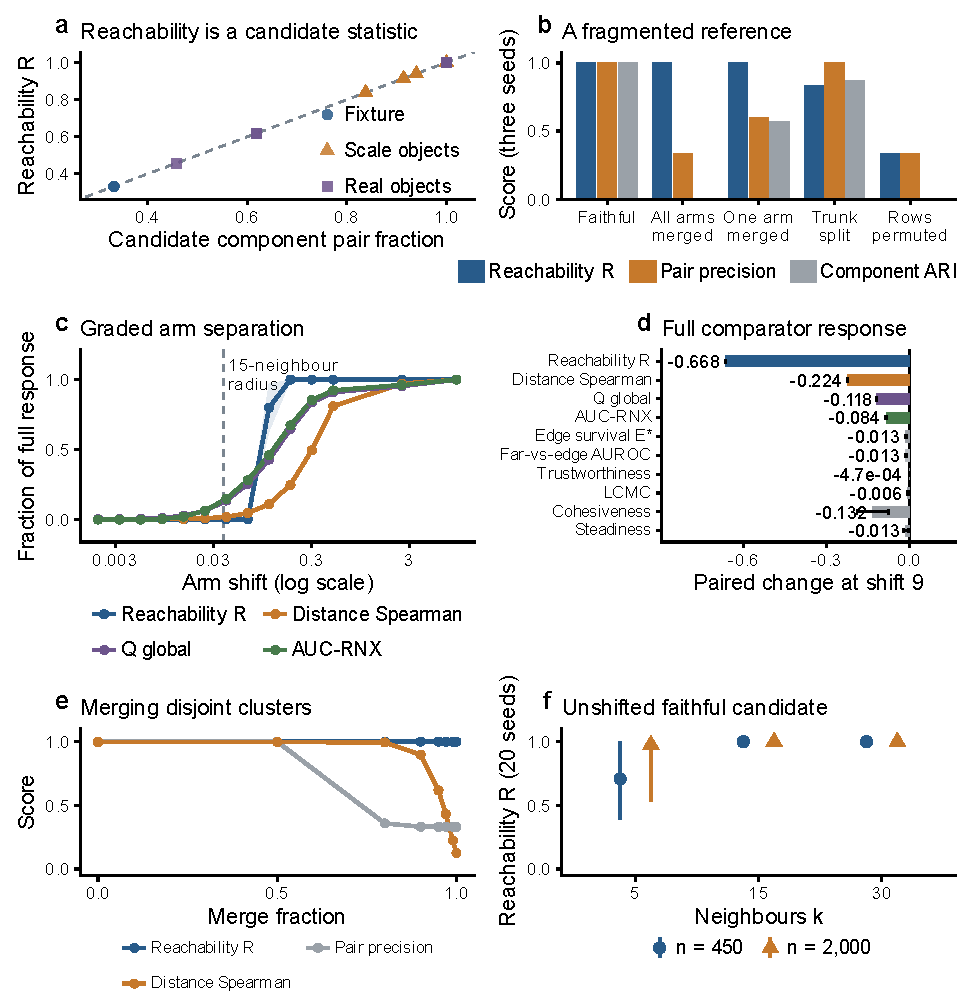
\includegraphics[width=\linewidth,height=0.74\textheight,keepaspectratio]{journal-figures/calibration_reachability.pdf}
\caption{What reachability measures. a, reachability against candidate component-pair fraction in the 322 connected-reference batteries; the dashed line is equality. b, a reference of three disjoint arms with five candidates (three-seed means): reachability ignores merging, which pair precision and component ARI detect. c, graded separation of the branching fixture ($n=450$, $k=15$, 20 seeds, independent candidate jitter); paired mean changes are divided by their mean response at shift 9. Ribbons show one seed standard deviation on that scale; the dashed line is the median reference 15th-neighbour distance. d, unnormalized paired mean changes at shift 9 for the complete displayed comparator set, with one-SD bars over the same seeds. e, merging three disjoint clusters by moving their centroids together, with seed-mean scores. f, reachability of the unshifted faithful candidate at three neighbour counts (points: seed means; bars: range over 20 seeds). Seed variability is fixture repeatability, not biological uncertainty.}
\label{fig:reachability}
\end{figure}


\FloatBarrier

Official graph connectivity conditions on branch labels, so it can remain high when the labelled arms are individually connected but disconnected from one another. That is compatible with its definition. A high root-order correlation can likewise coexist with changed branch geometry. The official trajectory score falls from 0.991--0.999 for faithful to 0.081--0.105 for matched shatter across the three seeds; complete collapse scores 0.527--0.560. The shatter response arises because the candidate graph splits into three components of one third of the cells each: the routine keeps one component and assigns the remaining cells zero pseudotime.

The identity control, whose coordinates equal the reference, scores only 0.383--0.391, and partial-collapse scores vary markedly across seeds (0.398, 0.991 and 0.964). These low values are not a root-selection artefact. In the three identity controls, the three complete collapses and one of the three partial collapses (seven cases in all), diffusion pseudotime orders the trunk correctly (within-branch Spearman 0.977--0.996) but reverses both arms ($-0.852$ to $-0.907$), whereas the faithful, noisier, rescaled and remaining partially collapsed candidates keep the correct direction in all three branches. In those seven cases the selected root lay at known pseudotime 0.06 or less, and substituting the cell of smallest known pseudotime changed the score by at most 0.010.

Independently of the official API, true-root diffusion pseudotime on the identity control depended on the diffusion settings: with three diffusion components instead of the default ten the score was 0.9995--0.9997 in all three seeds, with four components 0.33--0.34, and a 30-neighbour graph gave 0.9986--0.9995 where the 15-neighbour graph gave 0.383--0.391. In the same recomputation, added jitter of standard deviation 0.002 or 0.006 left the arms reversed in all 30 draws, whereas at 0.01 the arm order was restored in five of 15 draws; the stored faithful candidates, which carry jitter of that size, restored it in all three seeds.

The official trajectory value on this fixture therefore reports the stability of diffusion pseudotime on a nearly noise-free planar graph, not agreement between candidate and reference geometry. We retain the values without replacing the official calls by a preferred surrogate or generalizing them to other integration settings.

\subsection{Allocation coherence requires reference-aware baselines, native semantics and absolute variation}

Allocation coherence has to be read against a baseline of matched smoothness. Across the twelve native objects, unclipped coherence had median 0.812 (range 0.554--0.942). It exceeded raw Gaussian-mixture responsibilities fitted to the reference (median 0.643 for full covariance) and random smooth maps (0.335) in every object (\figpanel{fig:coherence}{a}). The three stored seeds of each background are separate points, and the raw mixture, fitted to the reference, has no coherence difference across those seeds. The saved graph-conditional bootstrap intervals for these raw-baseline differences were above zero. Raw mixtures are, however, sharper than the native allocations. Tempered to the same mean perplexity, the full-covariance mixture reached a median of 0.771, and native coherence exceeded it in only eight of twelve objects, by a median paired margin of 0.029; native allocations were higher in all three dentate and pancreas objects and lower in all three lung objects (\figpanel{fig:coherence}{c}). No bootstrap interval was computed for that tempered baseline. Among native objects, coherence tracked one minus Geary's $c$ with Spearman correlation 0.993 (\figpanel{fig:coherence}{b}), consistent with a Geary-type smoothness ratio rather than a distinct biological target. In the separate 200-draw unclipped analysis, about 47\% of null values were negative and observed coherence lay 13.8--70.6 null standard deviations above its null mean (\figpanel{fig:coherence}{d}). In the 999-draw permutation test reported below, $p=0.001$ is the resolution floor of the test, not an effect-size estimate.

\begin{figure}[tbp]
\centering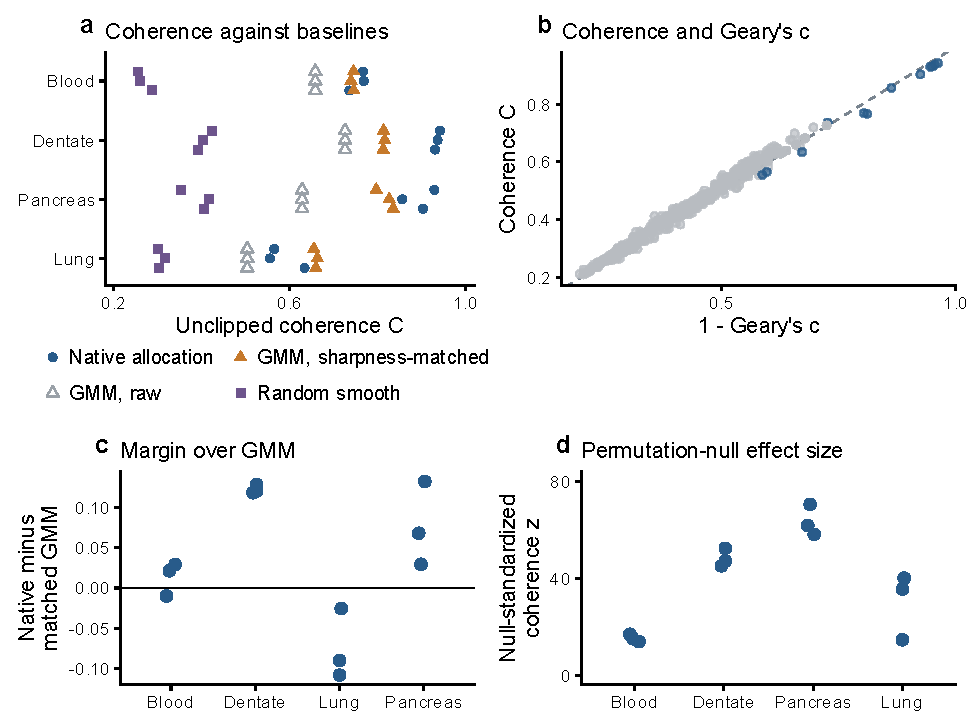
\includegraphics[width=\linewidth]{journal-figures/coherence_baselines.pdf}
\caption{Coherence against reference-aware baselines. a, unclipped coherence for twelve native objects, three stored seeds in each of four backgrounds, and three baselines: raw full-covariance Gaussian-mixture responsibilities on ten reference PCs, that mixture tempered to native mean perplexity, and the mean of 20 perplexity-matched random smooth maps. Vertical offsets separate stored seeds and have no quantitative meaning; horizontal position is coherence. The raw mixture is fitted to the reference, so its seeds have the same coherence. b, coherence against one minus multivariate Geary's $c$ on the same graph for native and raw-baseline allocations (native: blue; baselines: grey); the dashed line is equality. The reported association of 0.993 is restricted to the twelve native objects. c, native minus sharpness-matched mixture coherence by background; each point is one stored seed and the horizontal line is zero. d, native coherence standardized against its own 200-draw unclipped row-permutation null. Horizontal offsets separate stored seeds and have no quantitative meaning. No donor-level uncertainty or interval for the tempered mixture is implied.}
\label{fig:coherence}
\end{figure}



Coherence must also be read together with allocation dispersion. Raw coherence (\figpanel{fig:allocation}{a}) and normalized perplexity (\figpanel{fig:allocation}{b}) describe different properties. A smooth near-uniform allocation can have high raw coherence because both numerator and denominator are small. The guard withholds the quotable score. A constant allocation has no between-cell contrast; a uniform constant is also near-uniform. Sharp rows can be coherent or incoherent depending on their correspondence to the reference. Neither smoothness nor sharpness alone certifies a useful allocation.

\begin{figure}[tbp]
\centering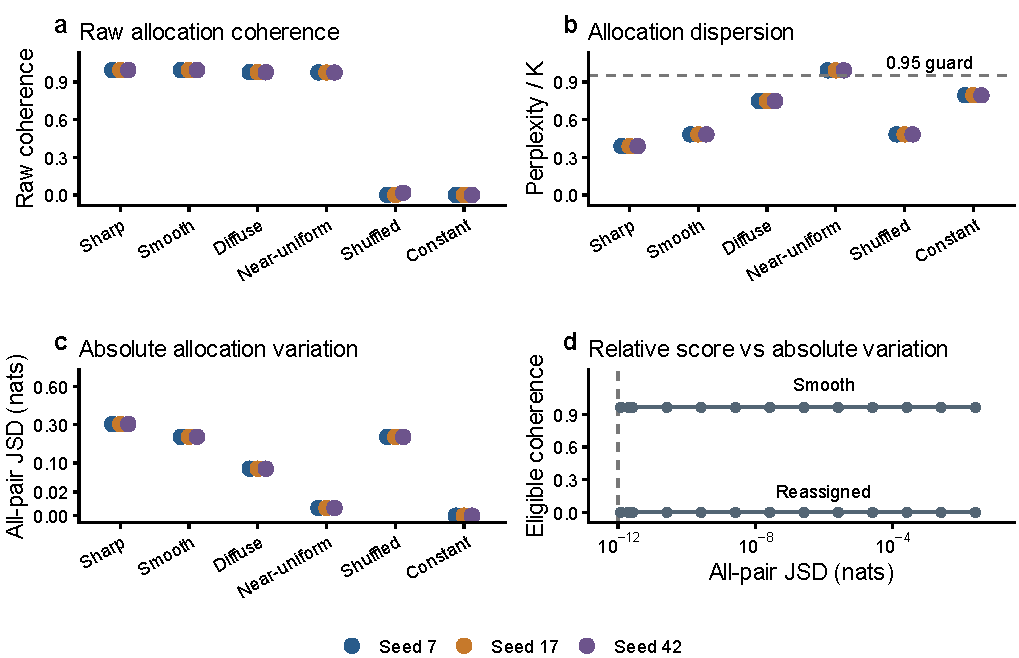
\includegraphics[width=\linewidth,height=0.64\textheight,keepaspectratio]{journal-figures/allocation_validity_guards.pdf}
\caption{Relative coherence, dispersion and absolute allocation variation. a, raw coherence for sharp, smooth, diffuse, near-uniform, shuffled and constant native controls. b, mean row perplexity divided by simplex dimension; the dashed 0.95 line marks the operational near-uniform guard. c, exact all-pair Jensen--Shannon divergence in nats on a square-root vertical axis. Coloured points and the shared seed key apply to a--c, retaining paired fixture seeds 7, 17 and 42 with horizontal offsets. Constant raw coherence is zero by guard convention. d, a separate independently validated 32-cell numerical fixture at $k=5$ varies tail mass in ten-coordinate probabilities $(1-\epsilon,\epsilon q_i)$ with smooth or bijectively reassigned nine-coordinate tails. Grey points show only numerically eligible cases; horizontal position is absolute all-pair divergence on a logarithmic axis, and the dashed line is the $10^{-12}$ denominator guard. Smooth coherence remains high across ten orders of absolute variation; reassignment reduces clipped coherence to zero. Guarded cases are retained in the numerical record but have no quotable ratio. The identity-explicit fixture implementation is distinct from the historical inventory scorer. Neither operational eligibility nor these synthetic replicates establishes biological usefulness or population-level uncertainty.}
\label{fig:allocation}
\end{figure}

The all-pair divergence exposes the absolute contrast hidden by the ratio (\figpanel{fig:allocation}{c}). The separate numerical tail fixture gives a more stringent counterexample (\figpanel{fig:allocation}{d}). Smooth allocations retain coherence 0.964 at both tail masses 1 and $10^{-10}$, while all-pair divergence falls from $2.65\times10^{-2}$ to $2.65\times10^{-12}$ nats and mean pairwise total variation from 0.158 to $1.58\times10^{-11}$. Both cases pass the declared numerical guards. Reassigning the same rows instead gives zero clipped coherence without changing all-pair divergence. Numerical eligibility therefore does not establish a useful allocation contrast. At smaller tail masses the degeneracy guard withholds coherence; those guarded cases remain in the full record rather than receiving artificial scores.



Across the historical inventory, \NativeFiles{} files contain native allocations: \ValidNativeFiles{} are quotable and \GuardedNativeFiles{} are guarded. The remaining \NonNativeFiles{} contain continuous coordinates (Supplementary Fig.~S2). Removing duplicate aliases yields \UniqueScores{} distinct computational objects: 752 valid native, 52 guarded native and 432 continuous (Supplementary Fig.~S2). Among the 804 distinct native objects, the largest absolute change from the re-executed historical sampled estimator is \MaxExactDelta{}. The mean signed change is 0.0006. Exact replacement therefore cannot be characterized as a machine-precision-only revision. Geometry definitions are unchanged. All \UniqueScores{} computations completed; the two excluded non-latent containers remain listed rather than silently dropped.

\subsection{Allocation eligibility changes the permutation-comparison denominator}

The focused manifest contains 60 native simplex allocations and 84 outputs with continuous coordinates. The latter comprise 48 mixture-regularized and 36 Gaussian variational controls. Native coherence is defined only for the \NullEligible{} quotable native allocations; the continuous outputs have no native coherence and do not enter its denominator. Of these allocations, \NullCoherence{} exceed all ten coherence permutations and \NullJoint{} exceed the edge, separation, and coherence maxima jointly (Supplementary Fig.~S2). Per-run margins preserve the unsuccessful comparison as well as the positive ones (Supplementary Fig.~S2). There are no near-uniform native rows in this focused manifest. The complete inventory does contain guarded native outputs; these are a different population.



\subsection{Dependence on graph scale and reference dimension}

The fixed sensitivity subset contains 24 computational objects: a native allocation and a continuous-coordinate representation for each of four backgrounds and three stored seeds. All nine combinations of $k\in\{5,15,30\}$ and reference dimension $d\in\{10,25,50\}$ are evaluated, giving 216 complete batteries. Absolute reachability is averaged across three stored seeds (Supplementary Fig.~S3); edge survival (Supplementary Fig.~S3), separation (Supplementary Fig.~S3) and native coherence (Supplementary Fig.~S3) show mean deviations from the same objects' $k=15,d=50$ baseline. Sixty of the 72 reachability group-setting changes are exactly zero, and all those absolute group means are one. This is a connectivity ceiling, not evidence of preserved row correspondence. Coherence is displayed only for the 12 native objects; continuous coordinates are structurally ineligible, not missing measurements. The candidate arrays are unchanged throughout this experiment.



Across the nine settings, median within-object score ranges are 0 for reachability, 0.312 for edge survival, and 0.135 for separation; the maximum reachability range is 0.162. For the 12 native objects, the median coherence range is 0.199, with range across objects 0.055--0.322. Much of the edge-survival range is a change in its chance level. Denser graphs shorten hop distances for any arrangement of rows, so the permutation expectation $E_0$ rose with $k$ in every object; the median within-object range of $E_0$ was 0.198, and from $k=5$ to $k=30$ the rise in $E_0$ matched a median 74\% of the rise in $E$ (\figpanel{fig:chance}{a}). After correction (Equation~\ref{eq:corrected}) the median within-object range was still 0.250 and, at the 50-PC reference, $E^*$ rose with $k$ in 23 of 24 objects (\figpanel{fig:chance}{b}), so the dependence on graph scale is real but smaller than the raw range suggests. Every candidate remained far above its own null (smallest $z=18$). Correction enlarged the setting dependence of separation (median range of $S^*$ was 0.256), and in one battery separation fell below its own null.

\begin{figure}[tbp]
\centering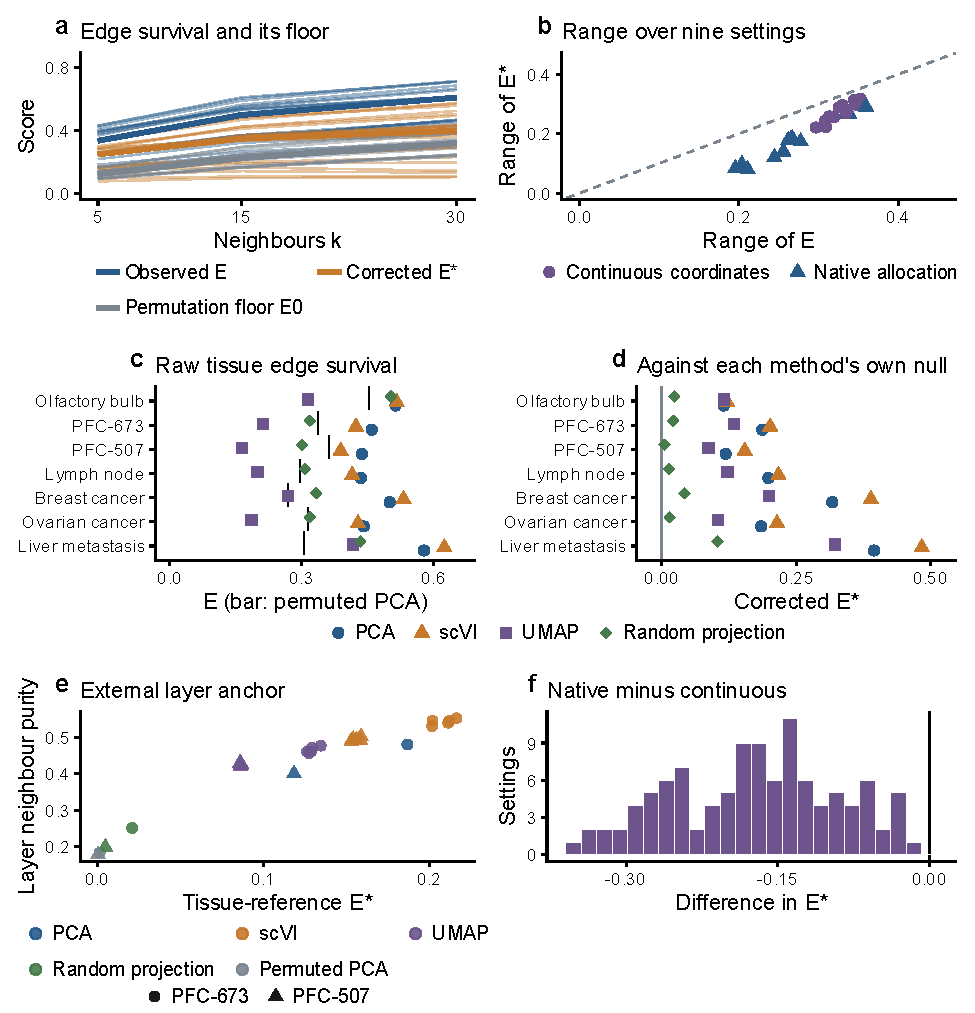
\includegraphics[width=\linewidth,height=0.74\textheight,keepaspectratio]{journal-figures/chance_correction.pdf}
\caption{Chance correction of edge survival. a, raw $E$, the 50-draw permutation mean $E_0$ and corrected $E^*$ against neighbour count for 24 scale objects at the 50-PC reference (thin lines: objects; thick lines: medians). b, within-object ranges over nine graph settings; the dashed line is equality. c, raw tissue-reference edge survival for regenerated candidates on seven sections; vertical bars mark permuted PCA. d, the same candidates corrected against their own 50-draw nulls. e, tissue-reference $E^*$ using exact candidate-pair expectations against candidate-neighbour cortical-layer purity on two prefrontal sections. Each section has thirteen plotted arrays: five scVI and five UMAP refits, plus PCA, random projection and permuted PCA; correlations exclude permuted PCA and use twelve arrays. f, native minus continuous corrected edge survival for all 108 matched settings. Arrays and settings are computational repeats, not independent biological units. Chance-correction panels use regenerated arrays, which reproduce the originally saved raw scores except for UMAP on one prefrontal section.}
\label{fig:chance}
\end{figure}

The paired-grid analysis asks a different question from the absolute-score ranges. All twelve native-minus-continuous edge differences retain their baseline sign across the nine settings, and the sign is the same everywhere: continuous coordinates score higher than the native allocations of the same background in 108 of 108 settings for $E$ and $E^*$ and 106 of 108 for $S$ (\figpanel{fig:chance}{f}); their median within-pair difference range is 0.060. Separation reverses in two of twelve pairs, both only at $k=5,d=10$ (dentate seed 0 and endocrinogenesis seed 1); its median difference range is 0.157. All twelve baseline reachability differences are exactly zero, so their absence of strict reversals is not a stable ordering. These comparisons are conditional on the fixed object pairs and do not isolate an effect of the native-allocation model.



{\looseness=1 {\looseness=1 {\looseness=1 {\looseness=1 In the separate 999-draw native permutation experiment, none of the twelve objects has a randomly reassigned-row coherence at or above its unpermuted coherence. The corrected Monte Carlo probability is therefore 0.001 for each object, the minimum attainable with 999 draws. The independent second stream again has zero exceedances for every object. Applying the declared post hoc twelve-test Holm correction to the original probabilities gives 0.012 for each object. Independent recomputation of all 216 graph settings agrees exactly with the archived values, with no exact neighbour-cutoff ties; the largest native-coherence discrepancy is $6.66\times10^{-16}$. The identity-explicit implementation reproduces all 444 archived batteries with no disagreement under the preset tolerances. The largest absolute difference from the archived values is 0 for reachability, $2.2\times10^{-16}$ for edge survival, 0 for separation and $1.6\times10^{-15}$ for native coherence. No object has a neighbour-cutoff tie or a zero-distance non-self pair, so these comparisons do not exercise the tie rule. Every joint-reorder control leaves the candidate and reference graphs unchanged, rotation with rescaling changes no geometry score, and both 999-draw streams again have zero exceedances for each of the twelve native objects. These checks support numerical reproducibility and the fixed-object correspondence result. They neither revise the historical 144-run counts nor establish a donor-level biological result.\par}\par}\par}\par}

\subsection{Row-correspondence damage leaves reachability unchanged by construction}

Because reassignment leaves the candidate graph connected, reachability must stay at one (Equation~\ref{eq:reachability} with a connected reference). For each native object, cyclic reassignment of selected rows preserves its exact multiset of allocations while damaging the alignment with reference cells. Five fractions and three corruption seeds give 180 batteries. Mean reachability is one at every fraction (Supplementary Fig.~S4). Mean edge survival declines from 0.374 to 0.198 (Supplementary Fig.~S4), separation from 0.704 to 0.520 (Supplementary Fig.~S4), and native coherence from 0.793 to 0.009 (Supplementary Fig.~S4) between intact and fully reassigned rows. Each panel retains background-specific curves and model-seed variation. The averages do not imply that every individual score decreases monotonically.



Forty-eight implementation controls rotate and uniformly rescale candidate coordinates or jointly reorder reference and candidate rows. Their largest absolute difference from the corresponding baseline, over the applicable geometry and coherence quantities, is $5.55\times10^{-16}$. Rotation is checked only for geometry because rotating a probability vector changes its allocation semantics. These controls support numerical invariance for the tested objects and software environment; they do not imply invariance to arbitrary reference changes.

The exact-tie stress test fails that invariance outside the stored population. The archived neighbour graph contains five self-loops for the twenty identical candidate rows. Joint row reordering changes edge survival by up to 0.0152 and separation by up to 0.1213 in absolute value, although reachability stays one. Duplicate coordinates make neighbour membership arbitrary, and positional self-removal is additionally unsafe. Thus an exactly collapsed representation needs an explicit identity-exclusion and tie policy before this implementation can support a permutation-invariant graph claim. The tie-free grid verification does not validate such an extension.

\subsection{Representation comparisons change once each candidate has its own null}

The six exported tissue views show olfactory bulb, prefrontal cortex, lymph node, breast cancer, ovarian cancer and liver metastasis in stored coordinates (\figpanel{fig:spatial}{a--f}). Breast-cancer spots (\figpanel{fig:views}{a--d}) and bulb spots (\figpanel{fig:views}{e--h}) are also drawn in tissue, PCA, UMAP and scVI coordinates, and the dissociated PBMC views have no tissue coordinate (Supplementary Fig.~S5). Against tissue position, expression PCA exceeds its row permutation on all seven sections in the archived record (\figpanel{fig:spatial}{g}; Supplementary Table~S2). In the regenerated arrays, raw edge survival places UMAP below permuted PCA on six of seven sections (\figpanel{fig:chance}{c}). That comparison mixes nulls: a two-dimensional UMAP graph has longer hop distances and a lower chance level than the higher-dimensional candidates (tissue $E_0$ 0.085--0.225 for UMAP against 0.23--0.50 for the others). Against its own permutation, UMAP exceeded its null and the corrected random projection on all seven sections ($E^*$ between 0.086 and 0.323), while ranking below scVI on seven and below PCA on six (\figpanel{fig:chance}{d}). After correction scVI matched or exceeded PCA on all seven sections, whereas raw scores placed PCA higher on four; the random projection fell from third to last, with $E^*$ between 0.004 and 0.104. The candidate ordering changed in 11 of 15 object--reference comparisons (pooled Kendall $\tau=0.46$ between raw and corrected scores). Five-seed scVI and UMAP refits on three sections had corrected tissue-edge-survival SDs of at most 0.0066, smaller than the scVI--PCA gaps on the prefrontal sections but not on the bulb, where their means and PCA lay within 0.115--0.123. On the two prefrontal sections, tissue-reference $E^*$ correlated descriptively with candidate-neighbour cortical-layer purity (Spearman 0.97 and 0.76 over twelve nonpermuted arrays per section), whereas raw $E$ did so more weakly (0.73 and 0.29) (\figpanel{fig:chance}{e}). These arrays include repeated seeds of two methods and do not supply independent donor-level replication.

\begin{figure}[tbp]
\centering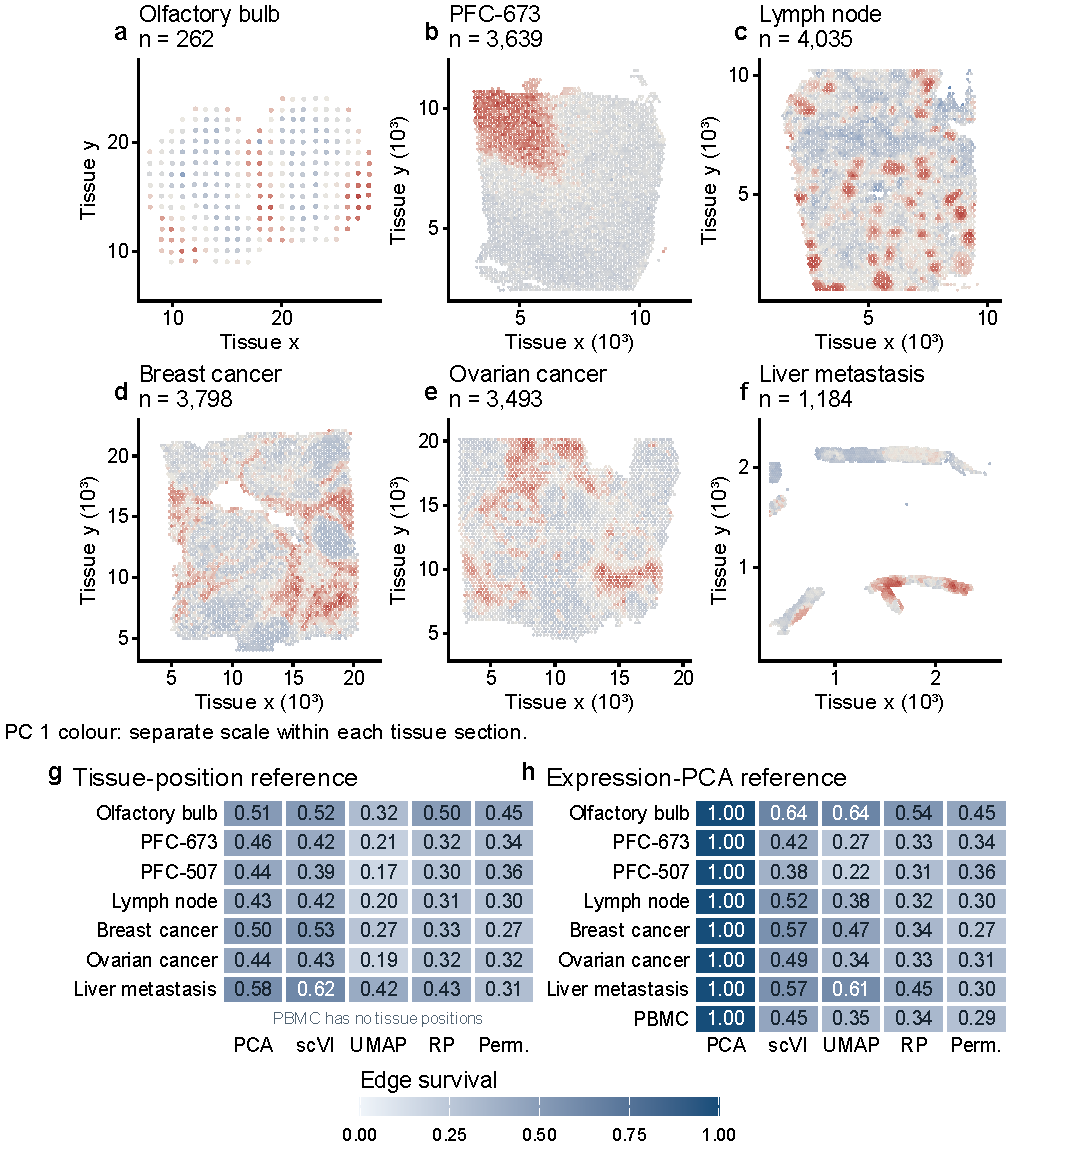
\includegraphics[width=\linewidth,height=0.76\textheight,keepaspectratio]{journal-figures/spatial_reference.pdf}
\caption{Tissue objects and the effect of declaring a reference. a, olfactory bulb. b, prefrontal section 151673. c, lymph node. d, breast cancer. e, ovarian cancer. f, liver metastasis. Stored tissue positions retain equal aspect; titles give spot counts. Axes marked $10^3$ express coordinates in thousands. Colour is expression PC 1 on a separate observed scale for each section, not a cell-type annotation. g, saved edge survival against tissue position for all seven evaluated sections, including prefrontal section 151507. h, saved edge survival against expression PCA for those sections and PBMC. Both matrices retain aligned section rows and the same method columns; RP denotes Gaussian random projection and Perm. PCA-row permutation. The unfilled bottom strip in g explains why PBMC has no spatial score: dissociated cells have no recorded tissue position, and no score is imputed. Annotations are rounded to two decimals on one zero-to-one colour scale; 1.00 is the edge-survival ceiling, meaning all reference edges remain candidate edges. PCA is 1 in h by construction because it is the declared expression reference. Each row is a fixed object, not donor-level replication.}
\label{fig:spatial}
\end{figure}

\begin{figure}[tbp]
\centering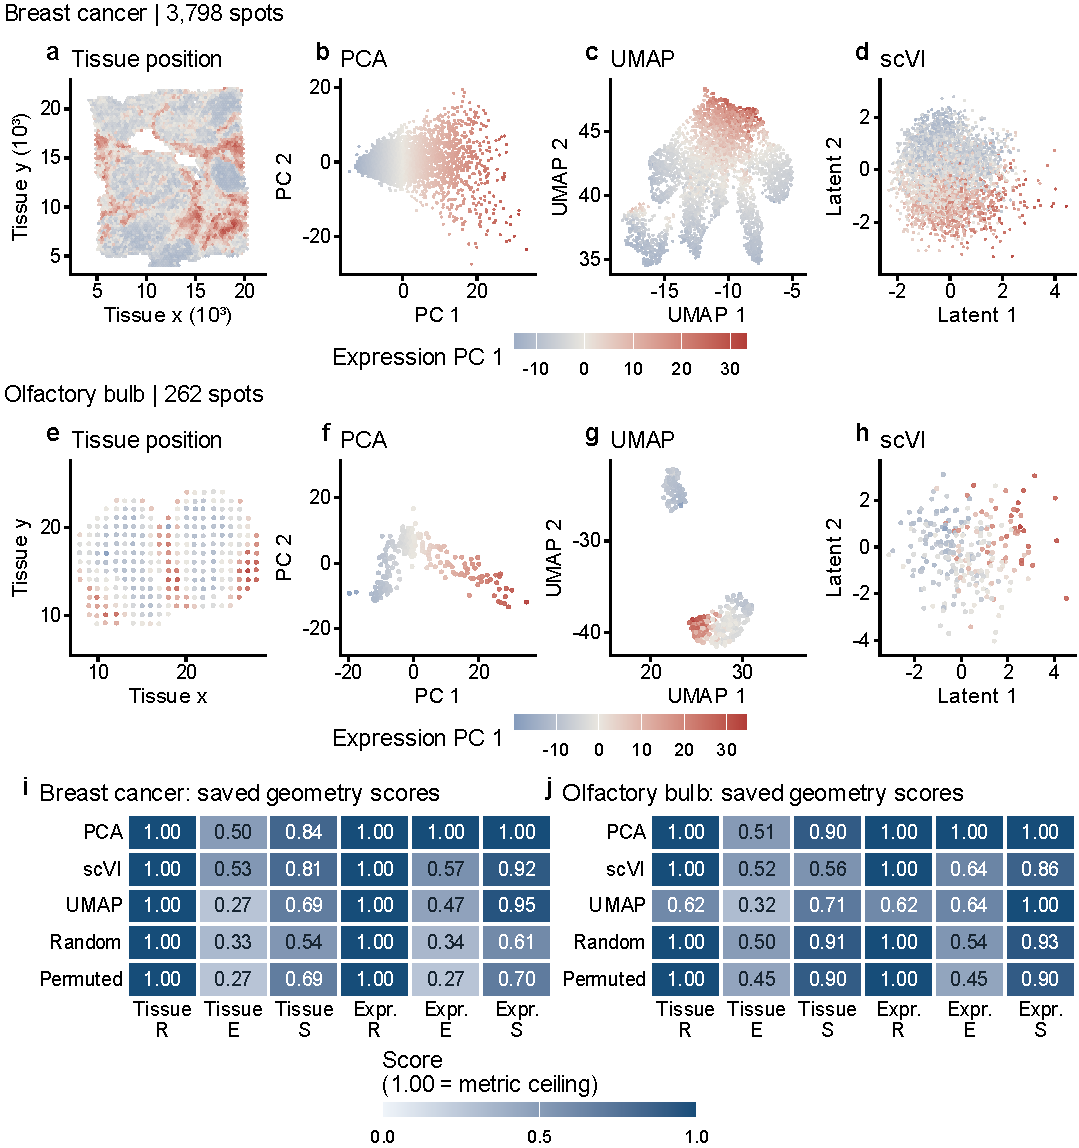
\includegraphics[width=\linewidth,height=0.74\textheight,keepaspectratio]{journal-figures/object_embeddings.pdf}
\caption{Coordinate views paired with saved geometry diagnostics. a, breast-cancer tissue position. b, the first two breast expression PCs. c, breast UMAP. d, the first two breast scVI latent dimensions. e, olfactory-bulb tissue position. f, the first two bulb expression PCs. g, bulb UMAP. h, the first two bulb scVI latent dimensions. All frames have equal coordinate aspect and use their own limits; breast tissue axes express stored coordinates in thousands. Expression PC 1 supplies one shared colour scale within each specimen; specimen scales differ. i, separately saved breast-cancer geometry diagnostics. j, separately saved bulb diagnostics. Columns show reachability R, edge survival E, and separation S against tissue position and expression PCA; rows retain PCA, scVI, UMAP, random projection, and row permutation. Scores are rounded to two decimals on one zero-to-one colour scale; a reachability value of 1.00 means that all reference-connected pairs remain connected, not that row correspondence is intact. The displayed scVI coordinates come from visualization refits under the recorded recipe and are not the scored latent arrays. These views are not tissue-boundary annotations, and the diagnostics are not biological ground truth.}
\label{fig:views}
\end{figure}

Exact distance ties in the tissue reference do not change these conclusions. Across the 62 reference graphs per section, edge survival varied by at most 0.0015 and corrected edge survival by at most 0.0021, reachability not at all, separation by at most 0.013 and corrected separation by at most 0.043; the tie-complete graph shifted corrected edge survival by at most 0.0017 and corrected separation by at most 0.040. Every ordering reported above held in every graph: UMAP above its null and above the random projection on all seven sections, scVI at or above PCA, the random projection last, UMAP below scVI on seven sections and below PCA on six, raw PCA above scVI on four, and the three liver-metastasis separation values below their nulls. Corrected edge survival ranged over 0.0867--0.3230 for UMAP and 0.0049--0.1038 for the random projection across all graphs.








\FloatBarrier

The paired breast and bulb score matrices preserve the archived raw diagnostics for both references (\figpanel{fig:views}{i--j}). Against the expression PCA, that PCA scores 1 by construction (\figpanel{fig:spatial}{h}; Supplementary Table~S3). Reachability below one for UMAP on the bulb (0.618) and on PBMC (0.457; Supplementary Fig.~S5) counts only the components of the UMAP graph itself. PBMC edge survival and separation (Supplementary Fig.~S5) are shown against their recorded PCA-row-permutation values; these raw displays do not replace candidate-specific chance correction. Separation did not give a reliable distinct diagnostic: its permutation expectation ranged from 0.50 to 0.91 across candidates, and PCA, scVI and UMAP on the liver-metastasis tissue reference all scored below their own separation null, whereas the random projection did not. These eight objects are still single sections or one blood matrix, not a population of donors.



\FloatBarrier

\section{Discussion}
The experiments support a conditional interpretation of geometric fidelity, and they show that the condition has to include the chance level of each score. Matching the starting noise removed an apparent local-score improvement under arm separation, and direct execution of the official trajectory API gave a strong shatter response that the local root-distance surrogate did not reproduce; those corrections address experimental confounding and implementation misidentification.

The second correction reverses several comparisons. Scored against its own permutation, UMAP retained tissue neighbourhoods above chance in edge survival on every section, and scVI matched or exceeded PCA on all seven fixed arrays, whereas raw edge survival placed PCA higher on four of the seven.

The same reasoning applies to allocation coherence. Native allocations exceeded random smooth and raw mixture baselines everywhere, but a mixture fitted to the reference and tempered to the same sharpness came close and exceeded them in lung.

Exact coherence improves one narrower aspect of reproducibility. Its denominator is a property of all distinct allocation pairs and therefore does not depend on which row positions happened to enter a random sample.

The stored-data census illustrates the importance of that eligibility denominator. Continuous coordinates, native allocations, guarded allocations, duplicate files, and repeated checkpoints all occur in the available collection.

Several design choices remain limitations of this measurement study. The archived calibration used identical reference and faithful noise draws; the graded calibration decoupled them and added three topologies without changing the conclusions, but all fixtures remain planar and noiseless in expression.

The practical implication is to make evaluation records more explicit. A reusable result should retain matched row identities, the reference construction, graph settings, the semantic type of the candidate, implementation versions, and unavailable or guarded outputs.

Biological validity needs an external target of its own. Count simulators such as Splatter~\cite{zappia2017splatter} and dynamic simulators such as dyngen~\cite{cannoodt2021dyngen} would extend the planar fixtures to realistic expression with known topology, and clonal lineage measurements~\cite{weinreb2020lineage} could test whether a corrected geometric score predicts observed fate.

\section{Declarations}

\section*{Data Availability}
The accompanying source bundle contains this revision's code, figure sources, saved score tables and the distributed candidate and reference arrays. The public repository is \url{https://github.com/PeterPonyu/reference-anchored-geometry}. The earlier software release is archived at \url{https://doi.org/10.5281/zenodo.22914409}; that immutable archive does not contain the present revision. The current analysis and document release is archived at \url{https://doi.org/10.5281/zenodo.23308078}. The bundle includes synthetic calibration arrays, 24 matched representation and reference arrays, seven tissue-section representations and one blood-sample representation, numerical tests and reproduction instructions. Public count matrices, complete expression caches, remaining historical latent files and the historical multi-library calibration driver are not redistributed; their source and reproduction limits are stated in the guide. Author-owned software is MIT licensed; author-owned research content is CC BY 4.0; third-party materials retain their original terms.

\section*{Code availability}
Analysis code, the identity-explicit scorer, saved calibration inputs and numerical validation are available at \url{https://github.com/PeterPonyu/reference-anchored-geometry} and archived at software DOI \url{https://doi.org/10.5281/zenodo.23308078}. The reproduction guide distinguishes saved-array analyses from steps requiring source count matrices or the historical calibration driver.

\noindent\textbf{Funding}\par\nobreak

This research received no funding.



\section*{Additional Information}
The author declares no competing interests.

{\footnotesize\raggedright\setlength{\bibsep}{1pt}\setlength{\emergencystretch}{3em}
\bibliographystyle{unsrtnat}
\bibliography{references}}

\section*{Author contributions}
Zeyu Fu is the sole author and was responsible for all aspects of the study and manuscript. Zeyu Fu is the corresponding contact for this manuscript.

\end{document}
